

\section{Введение}
Осциллограф является одним из важнейших исследовательских приборов. Чаще всего
он применяется для наблюдения и исследования переменных во времени электрических
сигналов.


\subsection{Задачи работы}


\begin{enumerate}
    \item Исследовать чувствительность пластин вертикального и горизонтального
отклонений осциллографической трубки.
    \item Наблюдать с помощью осциллографа синусоидальное напряжение, полученное с
выхода генератора.
        \item Получить фигуры Лиссажу и определить частоту исследуемого напряжения по
фигурам Лиссажу.

\end{enumerate}




\section{Основная часть}

\subsection{Теоретическая часть}
\subsubsection{Электронно-лучевая трубка}
Основным рабочим элементом осциллографа является электронно-лучевая трубка.
\parДля возникновения термоэлектронной эмиссии катод трубки нагревают, подавая на его нагреватель переменное напряжение. Высвободившиеся электроны ускоряются электрическим полем и движутся к аноду. На их пути расположен фокусирующий электрод, который формирует электроны в узкий пучок, создавая электронный луч. Совокупность нити накала, катода, фокусирующего электрода и анода называется электронной пушкой.
\parЭлектронный луч проходит через отверстие в аноде и попадает между пластинами двух взаимно перпендикулярных конденсаторов. При подаче напряжения:
\begin{enumerate}
    \item Первый конденсатор отклоняет луч в горизонтальном направлении.
   \item Второй конденсатор изменяет траекторию луча в вертикальном направлении.
\end{enumerate}
\parПосле прохождения отклоняющих пластин луч попадает в расширенную часть трубки, где ударяет в покрытый люминофором экран. Под воздействием электронов вещество экрана светится, создавая яркое пятно.
\parЕсли на пластины конденсатора С1 и С2  подать напряжение, то пятно на экране перемещается как в горизонтальном (вдоль оси х), так и вертикальном (вдоль
оси y) направлениях. При изменении напряжения на обоих конденсаторах пятно перемещается по некоторой траектории в плоскости экрана. 
\parПри подаче на конденсатор вертикального отклонения постоянного
напряжение пучок электронов, проходя через электрическое поле конденсатора, отклоняется под действием поля в вертикальном направлении. В итоге пятно на экране смещается вверх или вниз от первоначального положения. 
\parИзмерив напряжение $U_{(+-)}$ и вызванное им смещение $L_{(+-)}$, можно вычислить чувствительность пластин вертикального отклонения по следующей формуле:
\begin{equation}
    S_{y}=\frac{L_{(+-)}}{U_{(+-)} }(\frac{\text{мм}}{\text{В}})
\end{equation}
\parПри подаче на конденсатор переменного напряжения (например, синусоидального) пятно будет совершать гармонические колебания. При достаточной большой частоте f на экране будет наблюдаться светящаяся линия. Её размер $L_{\sim}$ будет соответствовать  двойной амплитуде приложенного напряжения. В этом случае чувствительность пластин осциллографа вычисляется по формуле:
\begin{equation}
\label{eq:2}
    S_{y}=\frac{L_{(+-)}}{2\sqrt{2}U_{eff} }(\frac{\text{мм}}{\text{В}}),
\end{equation}
где $U_{eff}$ - эффективное значение синусоидального напряжения($U_{eff}=\frac{U_0}{\sqrt{2}}$).
\parЕсли на конденсаторы подать на пластины от различных источников:
\begin{enumerate}
    \item На пластины горизонтального отклонения  $U_x=(U_0)_x*cos(2\pi{}f_x+\phi_x)$
   \item На пластины вертикального отклонения $U_y=(U_0)_y*cos(2\pi{}f_y+\phi_y)$,
\end{enumerate}
то на экране будет наблюдаться неустойчивое мелькающее изображение. Наблюдать неподвижную картинку можно только при определенном соотношении частот:
\begin{equation}
    f_{x}=nf_{y},
\end{equation}
 где n=1,2,$ \frac{1}{2}$,$ \frac{1}{3}$ и т.д. При таком соотношении на экране осциллографа можно наблюдать фигуры Лиссажу.
 \parПрименение в осциллографе электронно-лучевой трубки дает возможность
использовать осциллограф для наблюдения электрических сигналов, переменных во
времени. Пусть на пластины вертикального отклонения подается обычное синусоидальное напряжение и одновременно на пластины горизонтального отклонения подается пилообразное напряжение.
\parПри постоянном увеличении напряжения пятно движется по экрану слева направо с некоторой постоянной скоростью, зависящей от частоты развертки . Затем, когда напряжение быстро уменьшается, пятно практически мгновенно возвращается справа налево. Через интервал времени, равный периоду пилообразного напряжения, движение пятна повторяется.
\parОдновременно с этим пятно перемещается в вертикальном направлении под действием синусоидального напряжения. В случае, когда периоды напряжения удовлетворяют следующему соотношению: 
\begin{equation}
    T_{x}=nT_{y},
\end{equation}
где n=1,2,3 и т.д. картинка на экране окажется неподвижной.

\subsubsection{Блок-схема осциллографа}
Помимо электронно-лучевой трубки осциллограф состоит из следующих устройств: генератора "Развёртки", усилителей горизонтального и вертикального отклонения и других.



\subsection{Эксперимент}
Упрощённая блок-схема осциллографа представлена на рисунке ~\ref{fig:Упрощённая блок-схема}.

\begin{figure}[H]
\centering
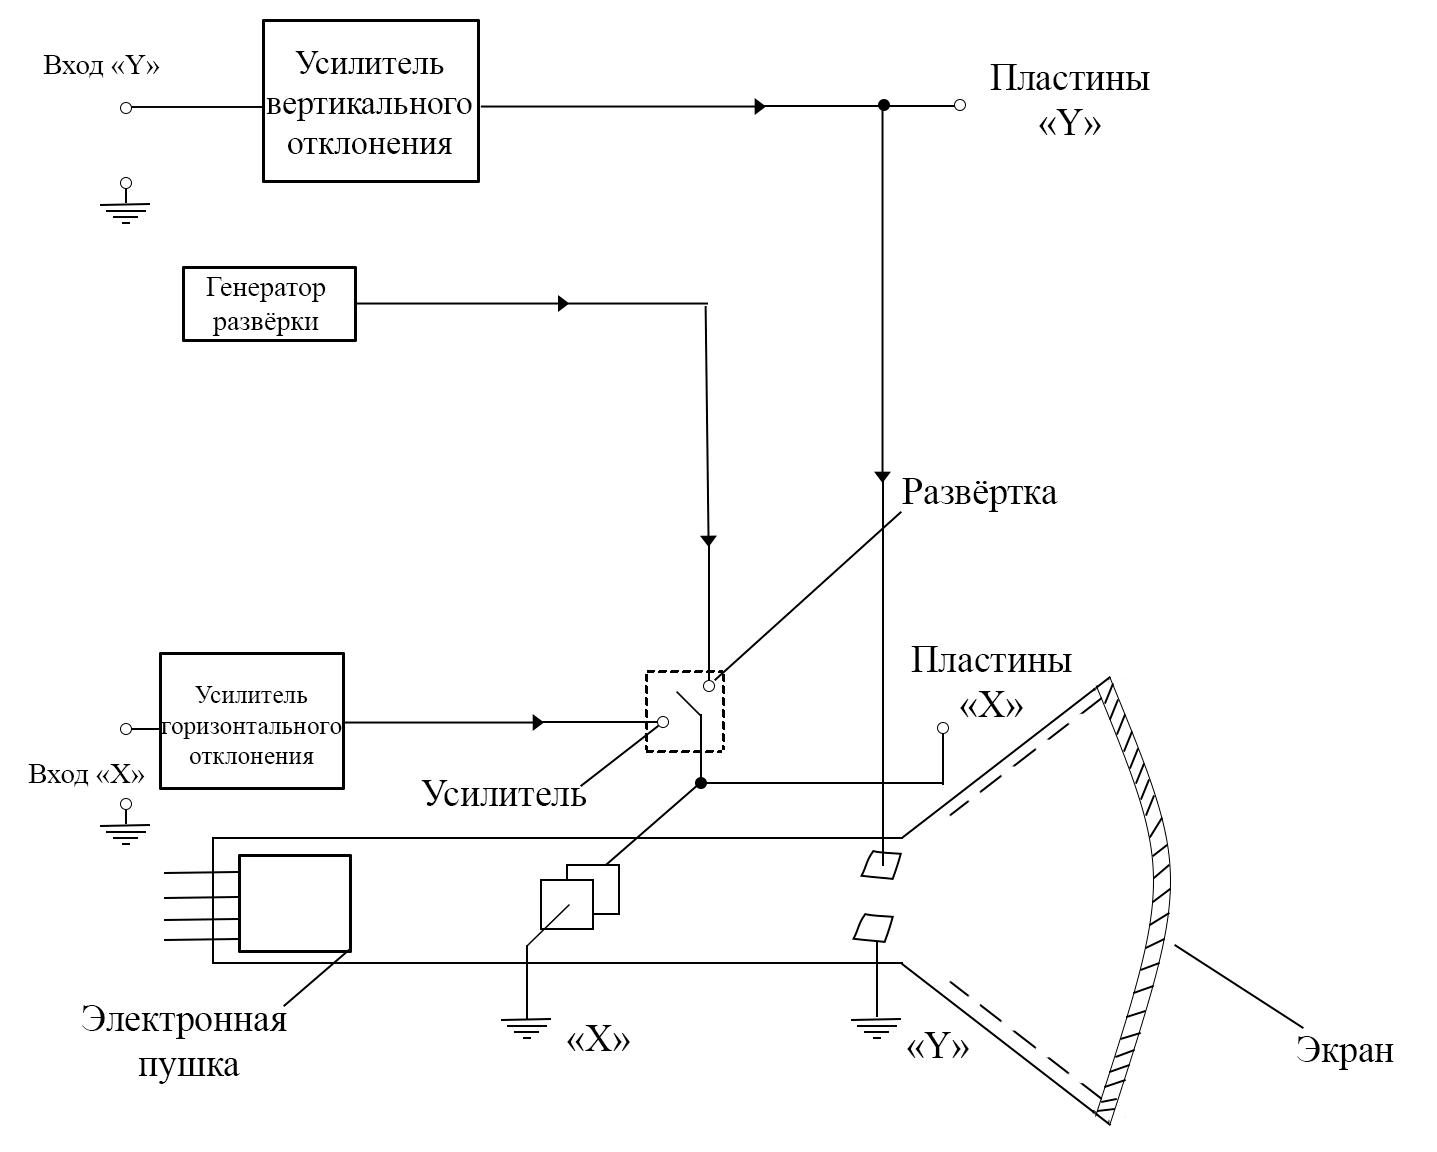
\includegraphics[width=1.0\textwidth]{Упрощённая блок-схема.png}
\caption{Схема электронно-лучевой трубки}
\label{fig:Упрощённая блок-схема}
\end{figure}

Фотография установки представлена на рисунке ~\ref{fig:Фотография установки}.

\begin{figure}[H]
\centering
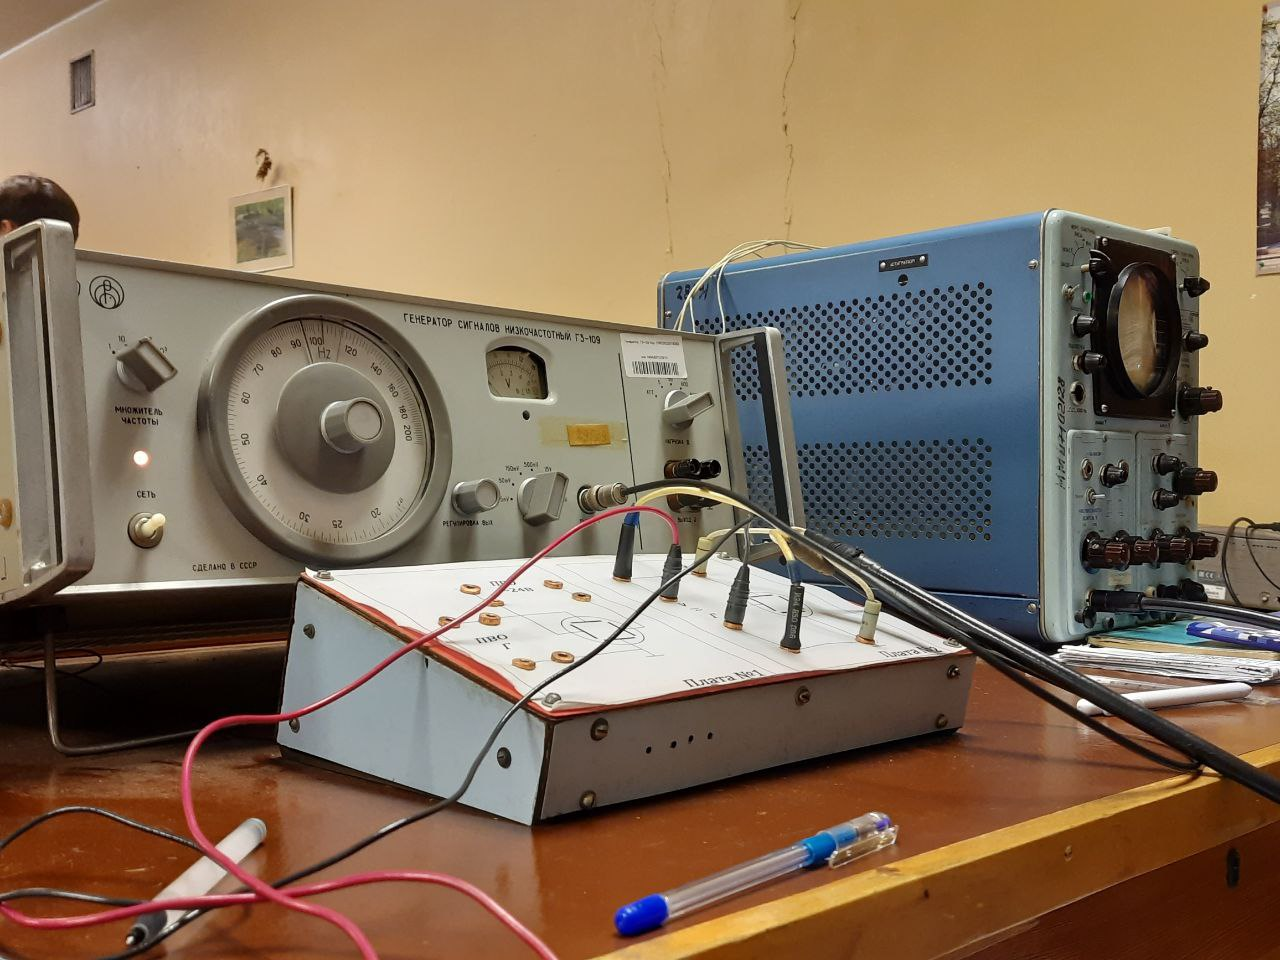
\includegraphics[width=1.0\textwidth]{Фотография установки.jpg}
\caption{Схема электронно-лучевой трубки}
\label{fig:Фотография установки}
\end{figure}

Одна из задач лабораторной работа заключается в исследовании чувствительности пластин вертикального и горизонтального отклонений электронно-лучевой трубки. На рисунке ~\ref{fig:Схема установки 1} представлена схема для исследования чувствительности пластин.
\parДругой задачей работы является наблюдение с помощью осциллографа синусоидального напряжения, полученного с выхода генератора. На рисунке ~\ref{fig:Схема установки 2} представлена схема для наблюдения исследуемого напряжения и определения максимальной чувствительности осциллографа.

\begin{figure}[H]
\centering
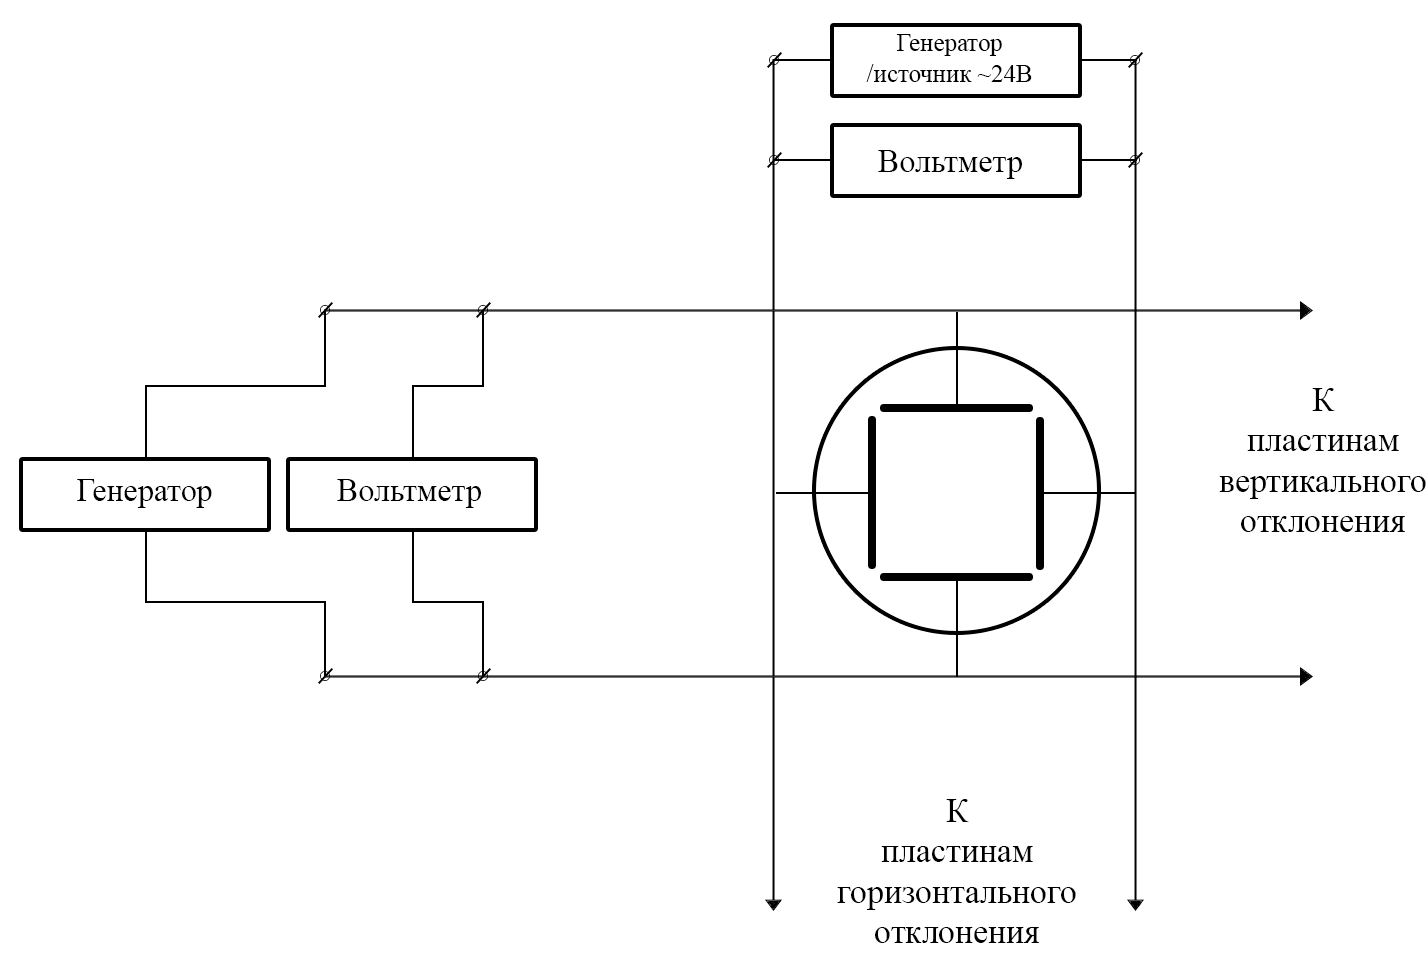
\includegraphics[width=0.9\textwidth]{Схема установки 1.png}
\caption{Схема электрической цепи для исследования чувствительности пластин
электронно-лучевой трубки и получения фигур Лиссажу}
\label{fig:Схема установки 1}
\end{figure}



\begin{figure}[H]
\centering
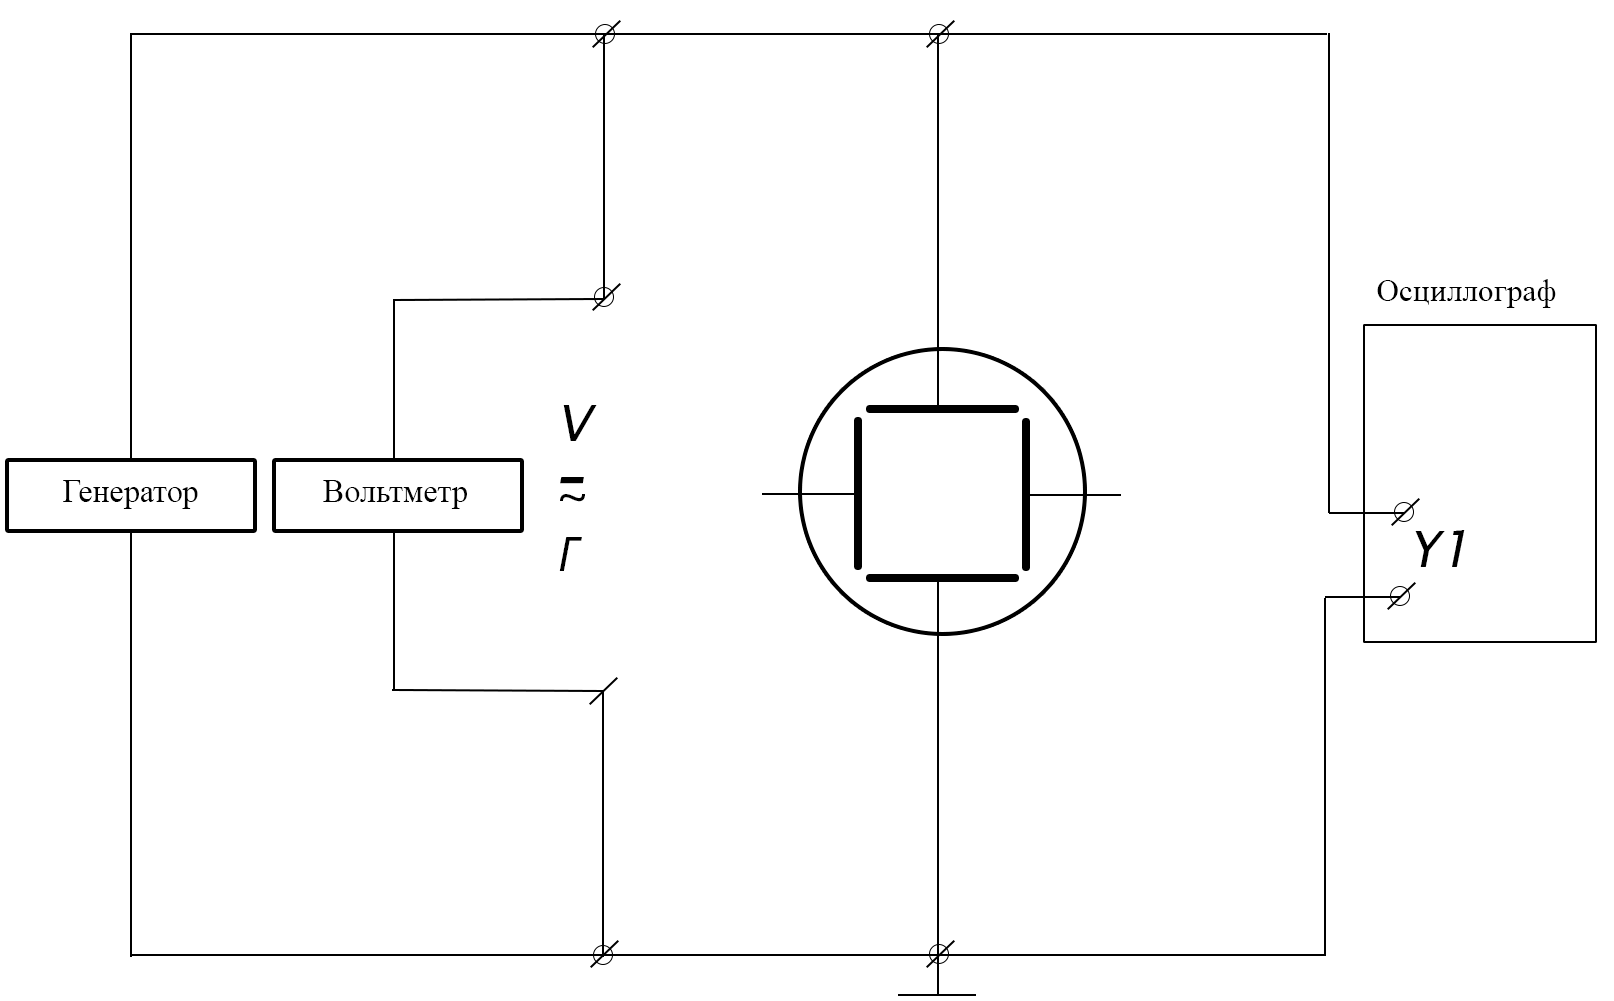
\includegraphics[width=0.9\textwidth]{Схема установки 2.png}
\caption{Схема электрической цепи для наблюдения исследуемого напряжения и
определения максимальной чувствительности осциллографа}
\label{fig:Схема установки 2}
\end{figure}


\subsection{Обработка данных и обсуждение результатов}
Чувствительность вычисляется по формуле (~\ref{eq:2})
\begin{center}
\begin{table}[h!]
\centering
\caption{Пластины вертикального отклонения (ПВО)}
\label{tabl:1}
\begin{tabular}{|c|c|c|c|}
\hline
\begin{minipage}{5cm}
\begin{center}
       Длина линии на экране, L
\end{center}
\end{minipage} &
\begin{minipage}{5cm}
\begin{center}
    Эффективное напряжение, $U_{eff}$
    \end{center}
\end{minipage} &
\begin{minipage}{5cm}
\begin{center}
    Чувствительность, S
\end{center}
\end{minipage}\\
\hline
мм&В&мм/В\\
\hline
10  &  5.50  &  0.64 \\
20  &  11.5  &  0.62\\
30  &  18.1  &  0.59 \\
40  &  24.5  &  0.58 \\
50  &  31.5  &  0.56 \\

\hline
\end{tabular}
\end{table}
\end{center}
Было высчитано среднее значение чувствительности пластин вертикального отклонения и погрешность результата прямых измерений по общепринятым правилам по отклонению от среднего:
\ $\overline{S_y}=0.60$ мм
\begin{center}
\begin{table}[h!]
\centering
\caption{Пластины горизонтального отклонения (ПГО)}
\label{tabl:1}
\begin{tabular}{|c|c|c|c|}
\hline
\begin{minipage}{5cm}
\begin{center}
    Длина линии на экране, L
\end{center}
\end{minipage} &
\begin{minipage}{5cm}
\begin{center}
    Эффективное напряжение, $U_{eff}$
    \end{center}
\end{minipage} &
\begin{minipage}{5cm}
\begin{center}
    Чувствительность, S
    \end{center}
\end{minipage}\\
\hline
мм&В&мм/В\\
\hline
10  &  4.70  &  0.75 \\
20  &  11.1  &  0.64\\
30  &  17.1  &  0.62 \\
40  &  24.1  &  0.59 \\
50  &  29.3  &  0.60 \\

\hline
\end{tabular}
\end{table}
\end{center}
Было высчитано среднее значение чувствительности пластин горизонтального отклонения и погрешность результата прямых измерений по общепринятым правилам по отклонению от среднего:
\ $\overline{S_x}=0.64$ мм
\parГрафики зависимости $S_y=f(U_{eff})$ и $S_x=f(U_{eff})$ представлены на рисунках и соотвествеенно.
\parМаксимальная чувствительность осциллографа вычисляется по формуле:
\begin{equation}
   (S^{'}_y)_m=\frac{L^{'}}{2\sqrt{2}U^{'}_{eff}},
\end{equation}
где $L^{'}$ - амплитуда синусоиды на экране осциллографа (двойная), в мм, $U^{'}_{eff}$ - напряжение, подаваемое на вход осциллографа и измеренное вольметром, в В.
\begin{center}
\begin{table}[h!]
\centering
\caption{Максимальная чувствительность осциллографа}
\label{tabl:1}
\begin{tabular}{|c|c|c|c|}
\hline
\begin{minipage}{5cm}
    Длина линии на экране, L
\end{minipage} &
\begin{minipage}{5cm}
    Эффективное напряжение, $U_{eff}$
\end{minipage} &
\begin{minipage}{5cm}
    Чувствительность, S
\end{minipage}\\
\hline
мм&В&мм/В\\
\hline
10  &  0.010 &  35*10 \\
20  &  0.023  &  31*10\\
30  &  0.037  &  29*10 \\
40  &  0.052  &  27*10 \\
50  &  0.064  &  28*10 \\
\hline
\end{tabular}
\end{table}
\end{center}
Был высчитан максимальный коэффициент усиления осциллографического усилителя по формуле:
\begin{equation}
   K_m=\frac{(\overline{S^{'}_y)_m}}{\overline{S^{}_y}},
\end{equation}
где $\overline{(S^{'}_y)_m}$ и $\overline{S^{}_y}$ среднее значение максимальной чувствительности осциллографа и среднее значение чувствительности пластин вертикального отклонения соотвественно. 


\begin{center}
\begin{table}[h!]
\centering
\caption{Измерение неизвестной частоты при наблюдении фигур Лиссажу}
\label{tabl:1}
\begin{tabular}{|c|c|c|c|c|}
\hline
\begin{minipage}{8cm}
\begin{center}
    Вид фигуры Лиссажу
\end{center}
\end{minipage} &
\begin{minipage}{2cm}
\begin{center}

\end{center}
\end{minipage} &
\begin{minipage}{2cm}
\begin{center}
    
    \end{center}
\end{minipage} &
\begin{minipage}{2cm}
\begin{center}

\end{center}
\end{minipage} &
\begin{minipage}{2cm}
\begin{center}
        
    \end{center}
\end{minipage}\\
\hline
Отношение частот  &  1:1 &  2:1 & 1:3 & 1:2 \\
Частота по лимбу генератора, $f_y$, Гц &  $50\pm{}0.5$  & $25\pm{}0.5$ & $150\pm{}0.5$ & $100\pm{}0.5$\\
Исследуемая частота, $f_x$, Гц  &  $50\pm{}0.5$  &  $50\pm{}0.5$ & $50\pm{}0.5$ & $50\pm{}0.5$ \\

\hline
\end{tabular}
\end{table}
\end{center}
\subsubsection{Исходный код}



\subsubsection{Графики}

На рис.~\ref{fig:graph1} приведён график зависимости результатов наблюдений от времени.
\begin{figure}[H]
\centering
\includegraphics[width=0.8\textwidth]{graph1}
\caption{Зависимость результатов наблюдений от времени}
\label{fig:graph1}
\end{figure}




\section{Выводы}



\begin{thebibliography}{9}

%ссылка на репозиторий с исходныим кодом отчета и всех расчетных программ 
\bibitem{repo}
\url{https://github.com/st117207/Workshop3}  (дата обращения: 10.04.2024) 


\end{thebibliography}

